% Ubah judul dan label berikut sesuai dengan yang diinginkan.
\section{Hasil dan Pembahasan}
\label{sec:hasildanpembahasan}

% Ubah paragraf-paragraf pada bagian ini sesuai dengan yang diinginkan.

% % Contoh input beberapa gambar pada halaman.
% \begin{figure*}
%     \centering
%     \subfloat[Hasil A]{\includegraphics[width=.4\textwidth]{example-image-a}
%         \label{fig:hasila}}
%     \hfil
%     \subfloat[Hasil B]{\includegraphics[width=.4\textwidth]{example-image-b}
%         \label{fig:hasilb}}
%     \caption{Contoh input beberapa gambar.}
%     \label{fig:hasil}
% \end{figure*}

% \lipsum[16-18]

% % Contoh input potongan kode dari file.
% \lstinputlisting[
%     language=Python,
%     caption={Program perhitungan bilangan prima.},
%     label={lst:bilanganprima}
% ]{program/bilangan-prima.py}

% \lipsum[19-20]

\subsection{Pengujian Bentuk Model}
\label{sec:analisismodel}
Bentuk model yang diujikan dilandaskan oleh bentuk model yang telah dijelaskan pada sub bab \ref{subsec:klasifikasipose}. Pengujian ini dilakukan untuk mengamati bagaimana pengaruh struktur model LSTM terhadap performa klasifikasi dari gerakan bahasa isyarat. Adapun perbedaan pada layer yang digunakan adalah sebagai berikut:

\begin{table}[H]
    \caption{Struktur Model LSTM}
    \label{tb:ringkasanModel}
    \centering
    \begin{tabular}{ll}
      \hline
      \textbf{Model} & \textbf{Struktur Layer} \\
      \hline
      Model 1 & 
      \begin{tabular}[t]{l}
        \emph{LSTM} 1 (128 unit, \emph{relu}) \\
        \emph{Dropout} 1 (0.5) \\
        \emph{LSTM} 2 (64 unit, \emph{relu}) \\
        \emph{Dropout} 2 (0.5) \\
      \end{tabular} \\
      \hline
      Model 2 & 
      \begin{tabular}[t]{l}
        \emph{TimeDistributed} (\emph{Dense}, 128 unit, \emph{tanh}) \\
        \emph{LSTM} 1 (64 unit, \emph{tanh}) \\
        \emph{Dropout} 1 (0.5) \\
      \end{tabular} \\
      \hline
      Model 3 & 
      \begin{tabular}[t]{l}
        \emph{TimeDistributed} (\emph{Dense}, 128 unit, \emph{tanh}) \\
        \emph{LSTM} 1 (128 unit, \emph{tanh}) \\
        \emph{Dropout} 1 (0.5) \\
        \emph{LSTM} 2 (64 unit, \emph{tanh}) \\
        \emph{Dropout} 2 (0.5) \\
      \end{tabular} \\
      \hline
    \end{tabular}
  \end{table}
  
Model dilatih dengan \emph{epoch} sebanyak 12 dengan partisi dataset sebesar 70:30, 70\% data training dan 30\% data validasi. Model yang telah dilatih kemudian diuji berdasarkan data testing yang ada dan memberikan hasil klasifikasi sebagai berikut:

\begin{table}[H]
    \caption{Hasil Evaluasi Model LSTM}
    \label{tb:evaluasiModel}
    \centering
    \begin{tabular}{llll}
      \hline
      \textbf{Model} & \textbf{\emph{Avg. Accuracy}} & \textbf{\emph{Avg. Precision}} & \textbf{\emph{Avg. F1-Score}} \\
      \hline
      Model 1 & 0.85 & 0.85 & 0.83 \\
      Model 2 & 0.94 & 0.94 & 0.94 \\
      Model 3 & 0.99 & 0.99 & 0.99 \\
      \hline
    \end{tabular}
  \end{table}
  
Berdasarkan tabel \ref{tb:evaluasiModel} dapat dilihat bahwa adanya relasi antara peningkatan kompleksitas dari model LSTM mempengaruhi performa klasifikasi gerakan bahasa isyarat. Hal ini dapat dilihat bahwa pada model ketiga menghasilkan performa terbaik dengan penggunaan \emph{layer} TimeDistributed dan 2 \emph{layer} LSTM.

\subsection{Pengujian Kondisi Cahaya}
\label{sec:analisiscahaya}

Pengujian ini akan dilihat bagaimana kemampuan adaptasi model terhadap perubahan intensitas cahaya dari ruangan. Pengujian ini dilakukan dengan menggunakan model ketiga yang telah diujikan pada tabel \ref{tb:ringkasanModel} dengan jarak pengguna 300 cm dari kamera. Pengambilan data intensitas cahaya dilakukan dengan aplikasi Lux Meter.

\begin{table}[H]
  \caption{Hasil Evaluasi Tingkat Cahaya}
  \label{tb:evaluasiCahaya}
  \centering
  \begin{tabular}{llll}
    \hline
    \textbf{Cahaya} & \textbf{Accuracy} & \emph{\textbf{Avg. Processing Time}} & \emph{\textbf{Avg. Complete Time}} \\
    \hline
    35 lux & 0.89 & 0.0938 & 3.0335 \\
    85 lux & 1.00 & 0.0918 & 2.9928 \\
    125 lux & 0.96 & 0.0923 & 2.4777 \\
    \hline
  \end{tabular}
\end{table}

Berdasarkan tabel \ref{tb:evaluasiCahaya} dapat dilihat bahwa adanya penurunan intensitas cahaya pada suatu ruangan menyebabkan adanya peningkatan pada \emph{processing time} dan \emph{complete time}. Namun apabila dilihat pada aspek akurasi, dapat dilihat bahwa intensitas cahaya 85 lux memiliki akurasi terbaik jika dibandingkan dengan intensitas cahaya lainnya. Hal ini dapat disebabkan oleh dataset yang digunakan memiliki intensitas cahaya yang memiliki nilai mendekati 85 lux.


\subsection{Pengujian Kondisi Jarak}
\label{sec:analisisjarak}

Pengujian ini akan dilihat bagaimana kemampuan adaptasi model terhadap perubahan jarak pengguna terhadap kamera.  Pengujian ini dilakukan dengan menggunakan model ketiga yang telah diujikan pada tabel \ref{tb:ringkasanModel} dengan intensitas cahaya bernilai 125 lux. Perlu diperhatikan bahwa gerakan isyarat pengguna dapat harus terlihat secara jelas pada kamera. 

\begin{table}[H]
  \caption{Hasil Evaluasi Jarak}
  \label{tb:evaluasiJarak}
  \centering
  \begin{tabular}{llll}
    \hline
    \textbf{Jarak} & \textbf{Accuracy} & \emph{\textbf{Avg. Processing Time}} & \emph{\textbf{Avg. Complete Time}} \\
    \hline
    180 cm & 0.89 & 0.1017 & 2.3660 \\
    240 cm & 0.96 & 0.0994 & 2.5098 \\
    300 cm & 1.00 & 0.0997 & 2.7918 \\
    \hline
  \end{tabular}
\end{table}

Berdasarkan tabel \ref{tb:evaluasiJarak} dapat dilihat bahwa peningkatan jarak menghasilkan klasifikassi model dengan akurasi yang lebih baik. Hal ini disebabkan oleh kemudahan kamera menangkap dengan jelas gerakan isyarat yang dilakukan oleh pengguna seiring dengan peningkatan jarak. Namun, peningkatan jarak mengakibatkan peningkatan pada \emph{complete time}. Pada \emph{processing time} cenderung bernilai fluktuatif.

\subsection{Pengujian Subjek Berbeda}
\label{sec:analisissubjek}

Pengujian ini dilakukan untuk melihat kemampuan adaptasi model terhadap perubahan subjek selain pengguna. Pengujian ini dilakukan dengan menggunakan model ketiga yang telah diujikan pada tabel \ref{tb:evaluasiModel} dengan intensitas cahaya bernilai 125 lux dan jarak terhadap kamera bernilai 300 cm. Subjek yang mengikuti pengujian ini dapat dlihat pada tabel \ref{tb:kondisisubjek}

\begin{table}[H]
  \caption{Variasi Subjek Berbeda}
  \label{tb:kondisisubjek}
  \centering
  \begin{tabular}{ll}
    \hline
    \textbf{Jenis Kelamin} & \textbf{Gambar Subjek} \\
    \hline
    Perempuan & 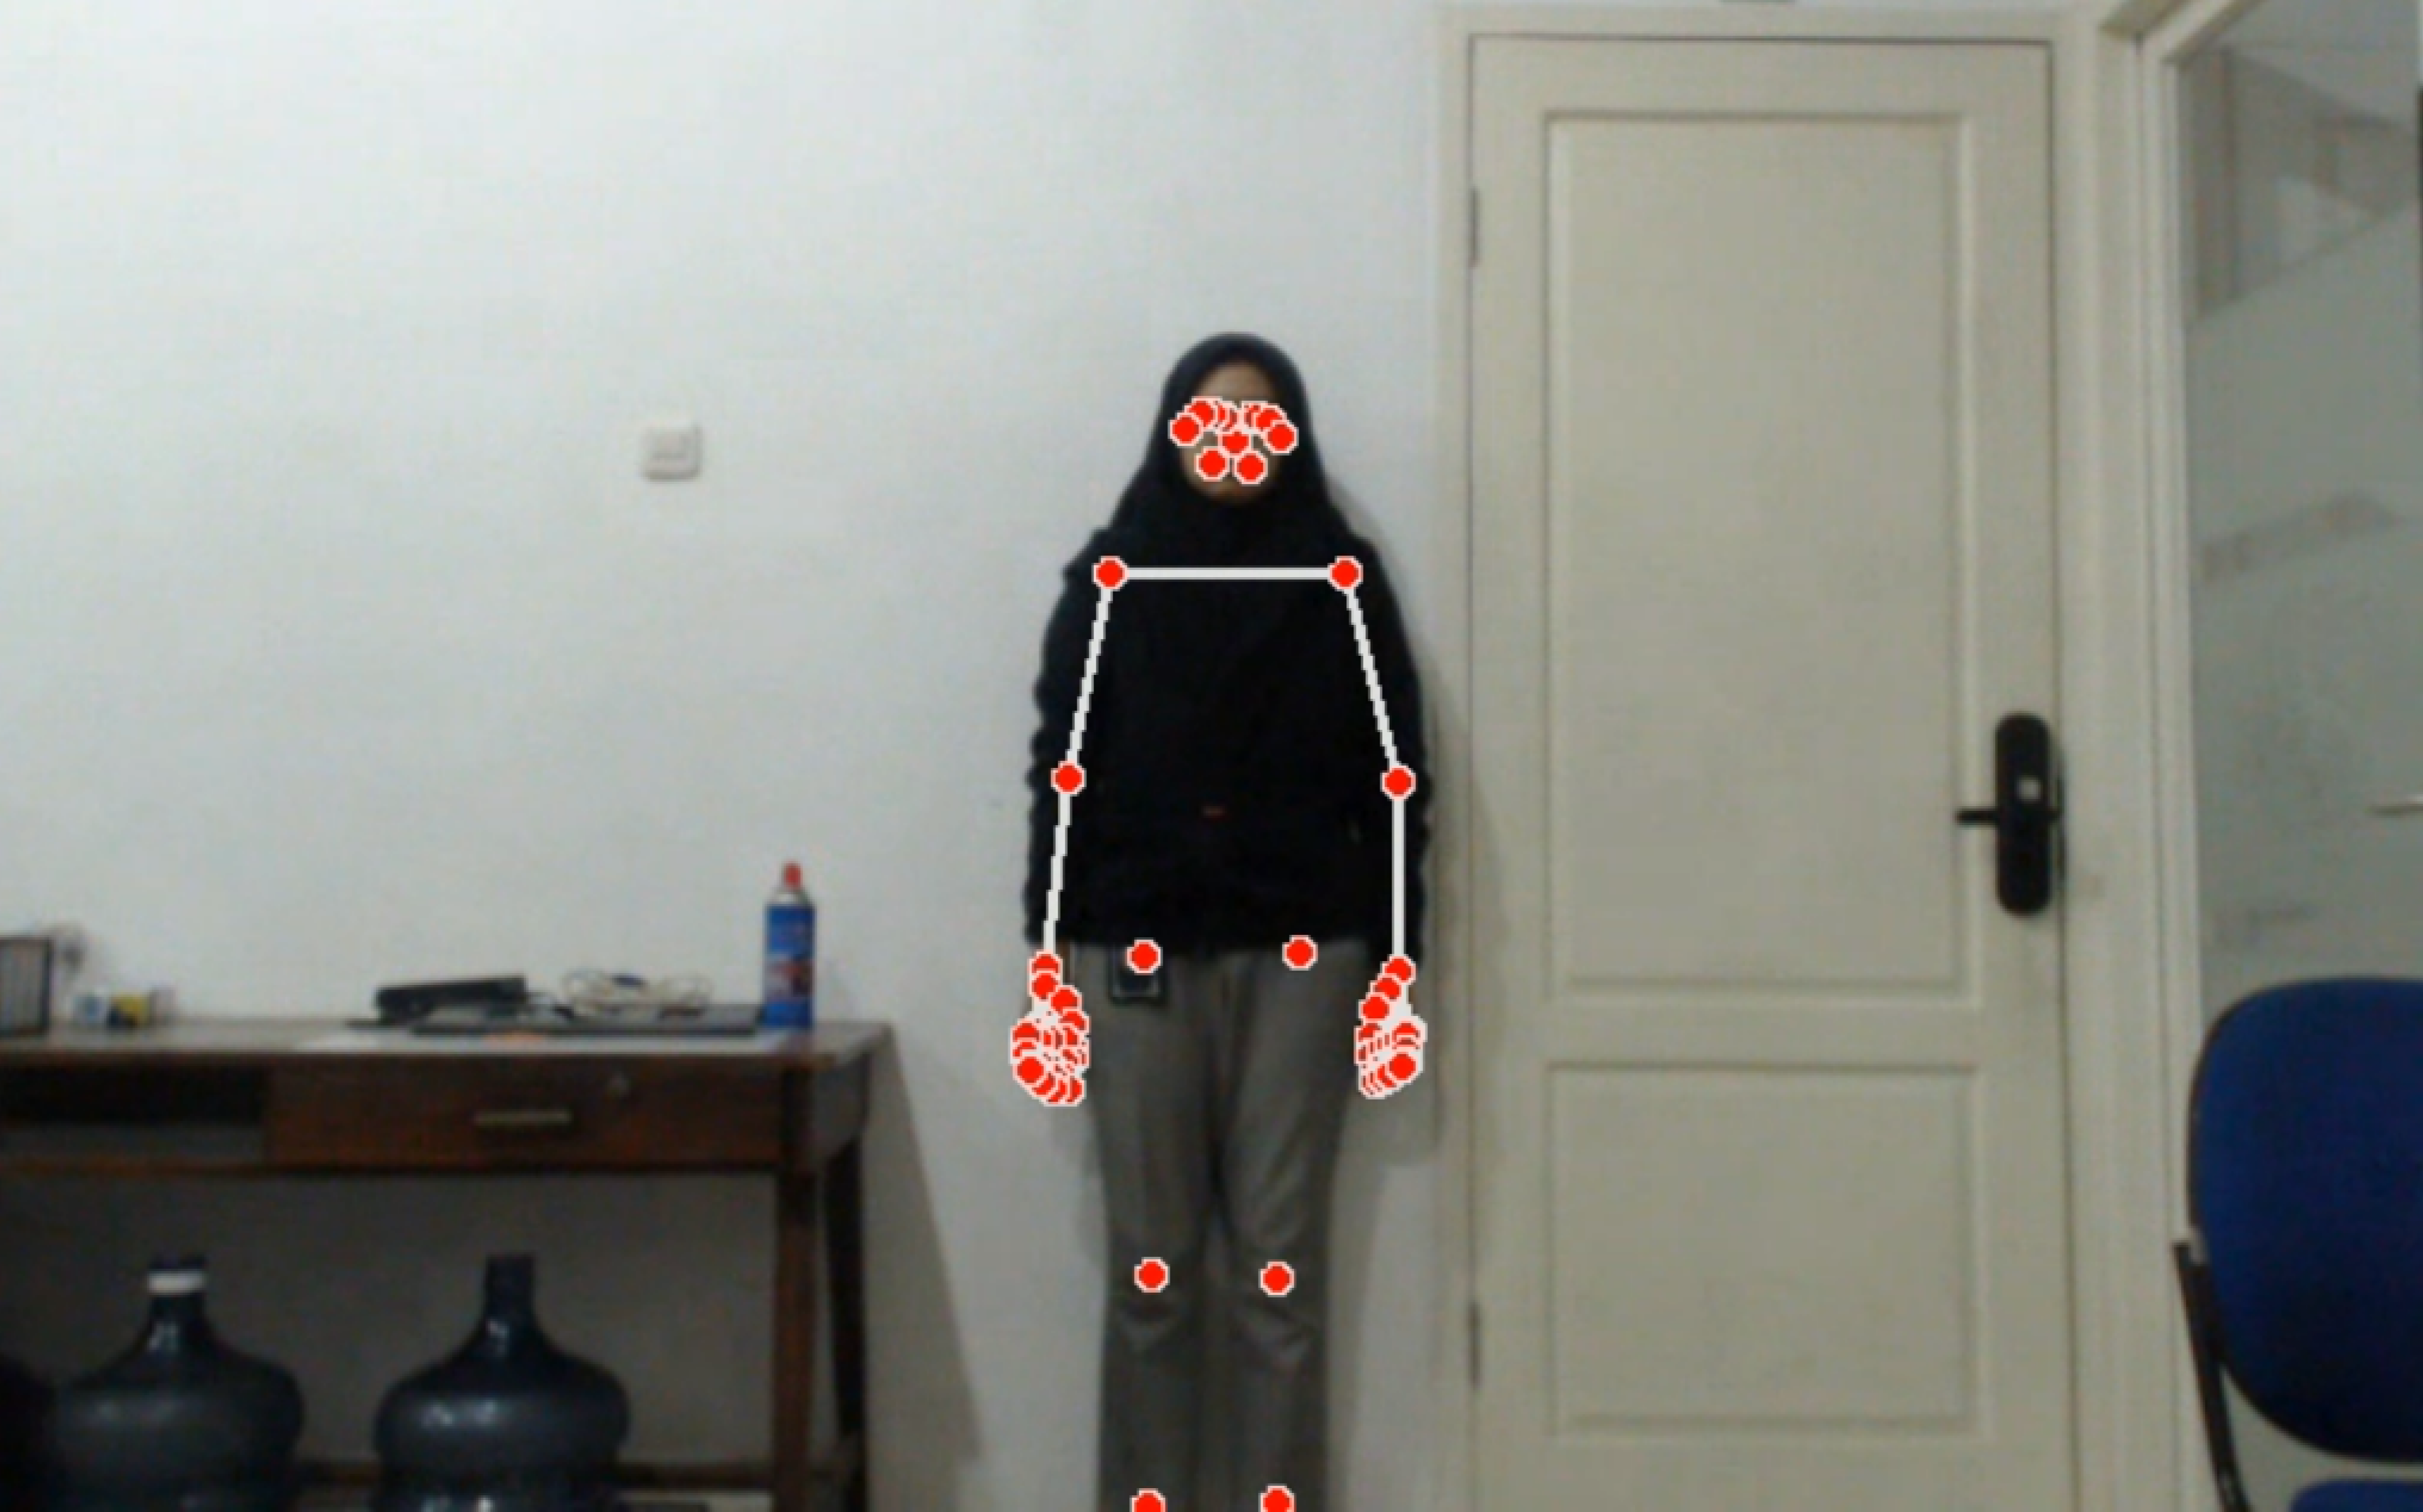
\includegraphics[scale=0.12]{gambar/bab4-rani.png} \\
    \hline
    Laki - Laki & 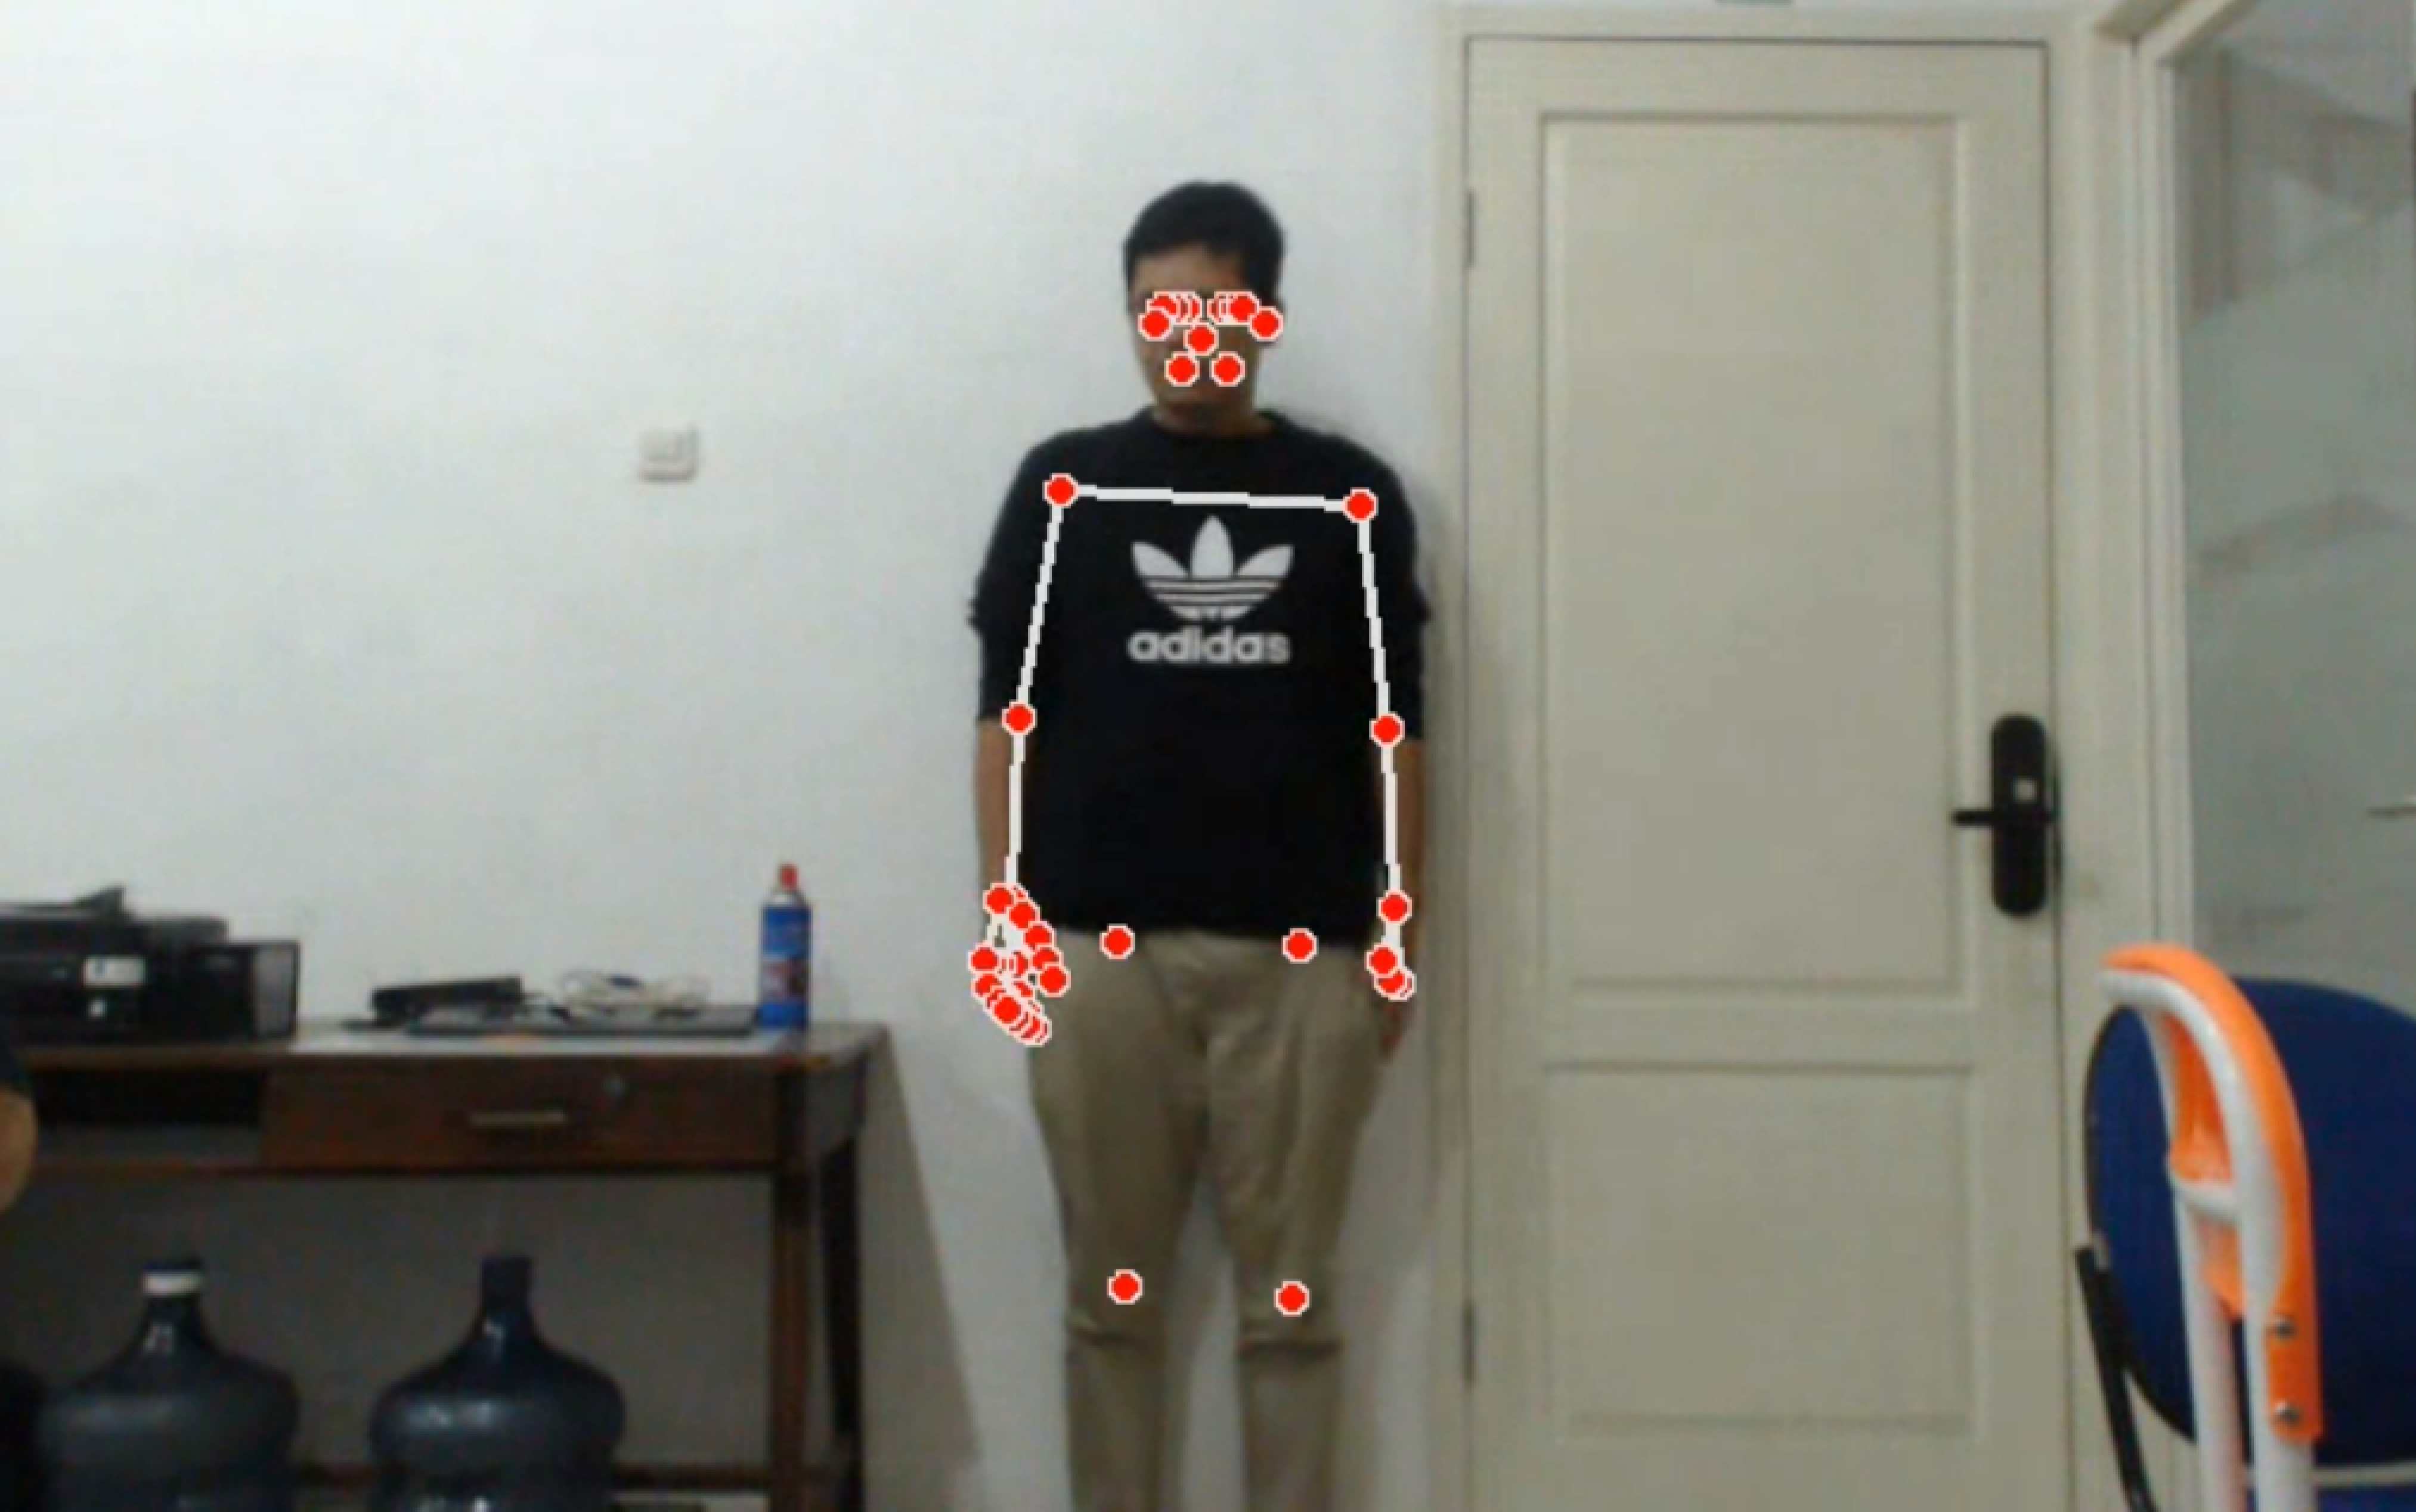
\includegraphics[scale=0.12]{gambar/bab4-evan.png} \\
    \hline
  \end{tabular}
\end{table}

\begin{table}[H]
  \caption{Hasil Evaluasi Subjek Berbeda}
  \label{tb:evaluasiSubjek}
  \centering
  \begin{tabular}{llll}
    \hline
    \textbf{Kombinasi} & \textbf{Accuracy} & \emph{\textbf{Avg. Processing Time}} & \emph{\textbf{Avg. Complete Time}} \\
    \hline
    Perempuan & 0.93 & 0.0988 & 2.6636 \\
    Laki - Laki & 0.93 & 0.0973 & 2.8191 \\
    \hline
  \end{tabular}
\end{table}

Berdasarkan tabel \ref{tb:evaluasiSubjek} dapat dilihat bahwa model dapat melakukan klasifikasi pada subjek yang berbeda. Normalisasi data telah menghasilkan model yang \emph{scale invariant} dan \emph{position invariant}. Adapun akurasi klasifikasi model menunjukkan nilai yang sangat baik, yaitu bernilai 0.93 atau 93\%. \emph{Average processing time} dan \emph{complete time} juga menunjukkan nilai yang tidak jauh dengan pengujian yang dilakukan oleh penulis sebelumnya, yaitu untuk \emph{average processing time} berkisar pada 0.098 dan untuk \emph{complete time} berkisar pada 2.74. 

\subsection{Pengujian Pembentukan Kalimat dan Konversi Suara}
\label{sec:analisiskalimat}

Pengujian ini dilakukan untuk memahami bagaimana sistem penerjemah digunakan untuk membentuk serangkaian kalimat dan melakukan konversi suara berdasarkan kalimat yang dibentuk. Dalam membentuk kalimat pada sistem ini merujuk pada sub bab \ref{subsec:sisitemkontrol}. Kalimat akan dibentuk berdasarkan kombinasi dari kosakata yang terdeteksi. Kombinasi kosakata secara lengkap pada tabel \ref{tb:kombinasiKosakata}. Pengujian ini dilakukan dengan menggunakan model ketiga yang telah diujikan pada tabel \ref{tb:evaluasiModel} dengan intensitas cahaya bernilai 125 lux dan jarak terhadap kamera bernilai 300 cm. Maksimal perulangan yang dilakukan adalah sebanyak 3 kali untuk masing - masing kosakata. Untuk setiap kombinasi kosakata juga dilakukan pengujian terhadap kosakata kontrol, meliputi "standby", "\emph{delete}", dan "\emph{translate}".

\begin{table}[H]
  \caption{Kombinasi Kosakata dan Kalimat}
  \label{tb:kombinasiKosakata}
  \centering
  \begin{tabular}{ll}
    \hline
    \textbf{Kombinasi Kosakata} & \textbf{Kalimat} \\
    \hline
    "Maaf" + "Siapa" + "Nama" & "Maaf siapa nama kamu?" \\
    "Maaf" + "Tolong" + "Saya" & "Maaf tolong bantu saya" \\
    "Maaf" + "Rumah" + "Siapa" & "Maaf ini rumah siapa?" \\
    "Rumah" + "Saya" & "Ini rumah saya" \\
    "Rumah" + "Siapa" & "Ini rumah siapa?" \\
    "Siapa" + "Nama" & "Siapa nama kamu?" \\
    "Tolong" + "Saya" & "Tolong bantu saya" \\
    \hline
  \end{tabular}
\end{table}


\begin{table}[H]
  \caption{Hasil Evaluasi Kombinasi Kosakata}
  \label{tb:evaluasiKombinasi}
  \centering
  \begin{tabular}{llll}
    \hline
    \textbf{Kombinasi} & \textbf{Accuracy} & \emph{\textbf{Avg. Processing Time}} & \emph{\textbf{Avg. Complete Time}} \\
    \hline
    2 kosakata & 1.00 & 0.0993 & 2.8303 \\
    3 kosakata & 0.93 & 0.0981 & 2.0513 \\
    \hline
  \end{tabular}
\end{table}

Dapat dilihat pada tabel \ref{tb:evaluasiKombinasi} bahwa model telah berhasil membentuk kalimat dengan melakukan kombinasi secara sekuensial dan berkelanjutan. Hal ini ditunjukkan dengan akurasi pada kalimat yang dibentuk dari kombinasi 2 kosakata bernilai 1.00 dan kombinasi 3 kosakata bernilai 0.93. Untuk nilai \emph{average processing time} dan nilai \emph{average complete time} tidak mengalami perubahan yang signifikan dengan pengujian yang berjalan secara berkelanjutan. Adapun dalam pembentukan kalimat "Ini rumah saya", terdapat kesalahan dalam klasifikasi gerakan isyarat "rumah" yang diklasifikasikan sebagai "delete". Hal ini disebabkan oleh tingkat kemiripan yang cukup tinggi antara gerakan isyarat "rumah" dan "delete". Secara keseluruhan, tingkat keberhasilan sistem dalam membentuk kalimat adalah 0.857 atau 85.7\%.

Berdasarkan keseluruhan pengujian yang dilakukan menunjukkan bahwa sistem memiliki performa yang baik dalam penerjemahan gerakan isyarat dalam jumlah yang relatif banyak dan secara \emph{realtime}.

\begin{figure}[ht]
    \centering

    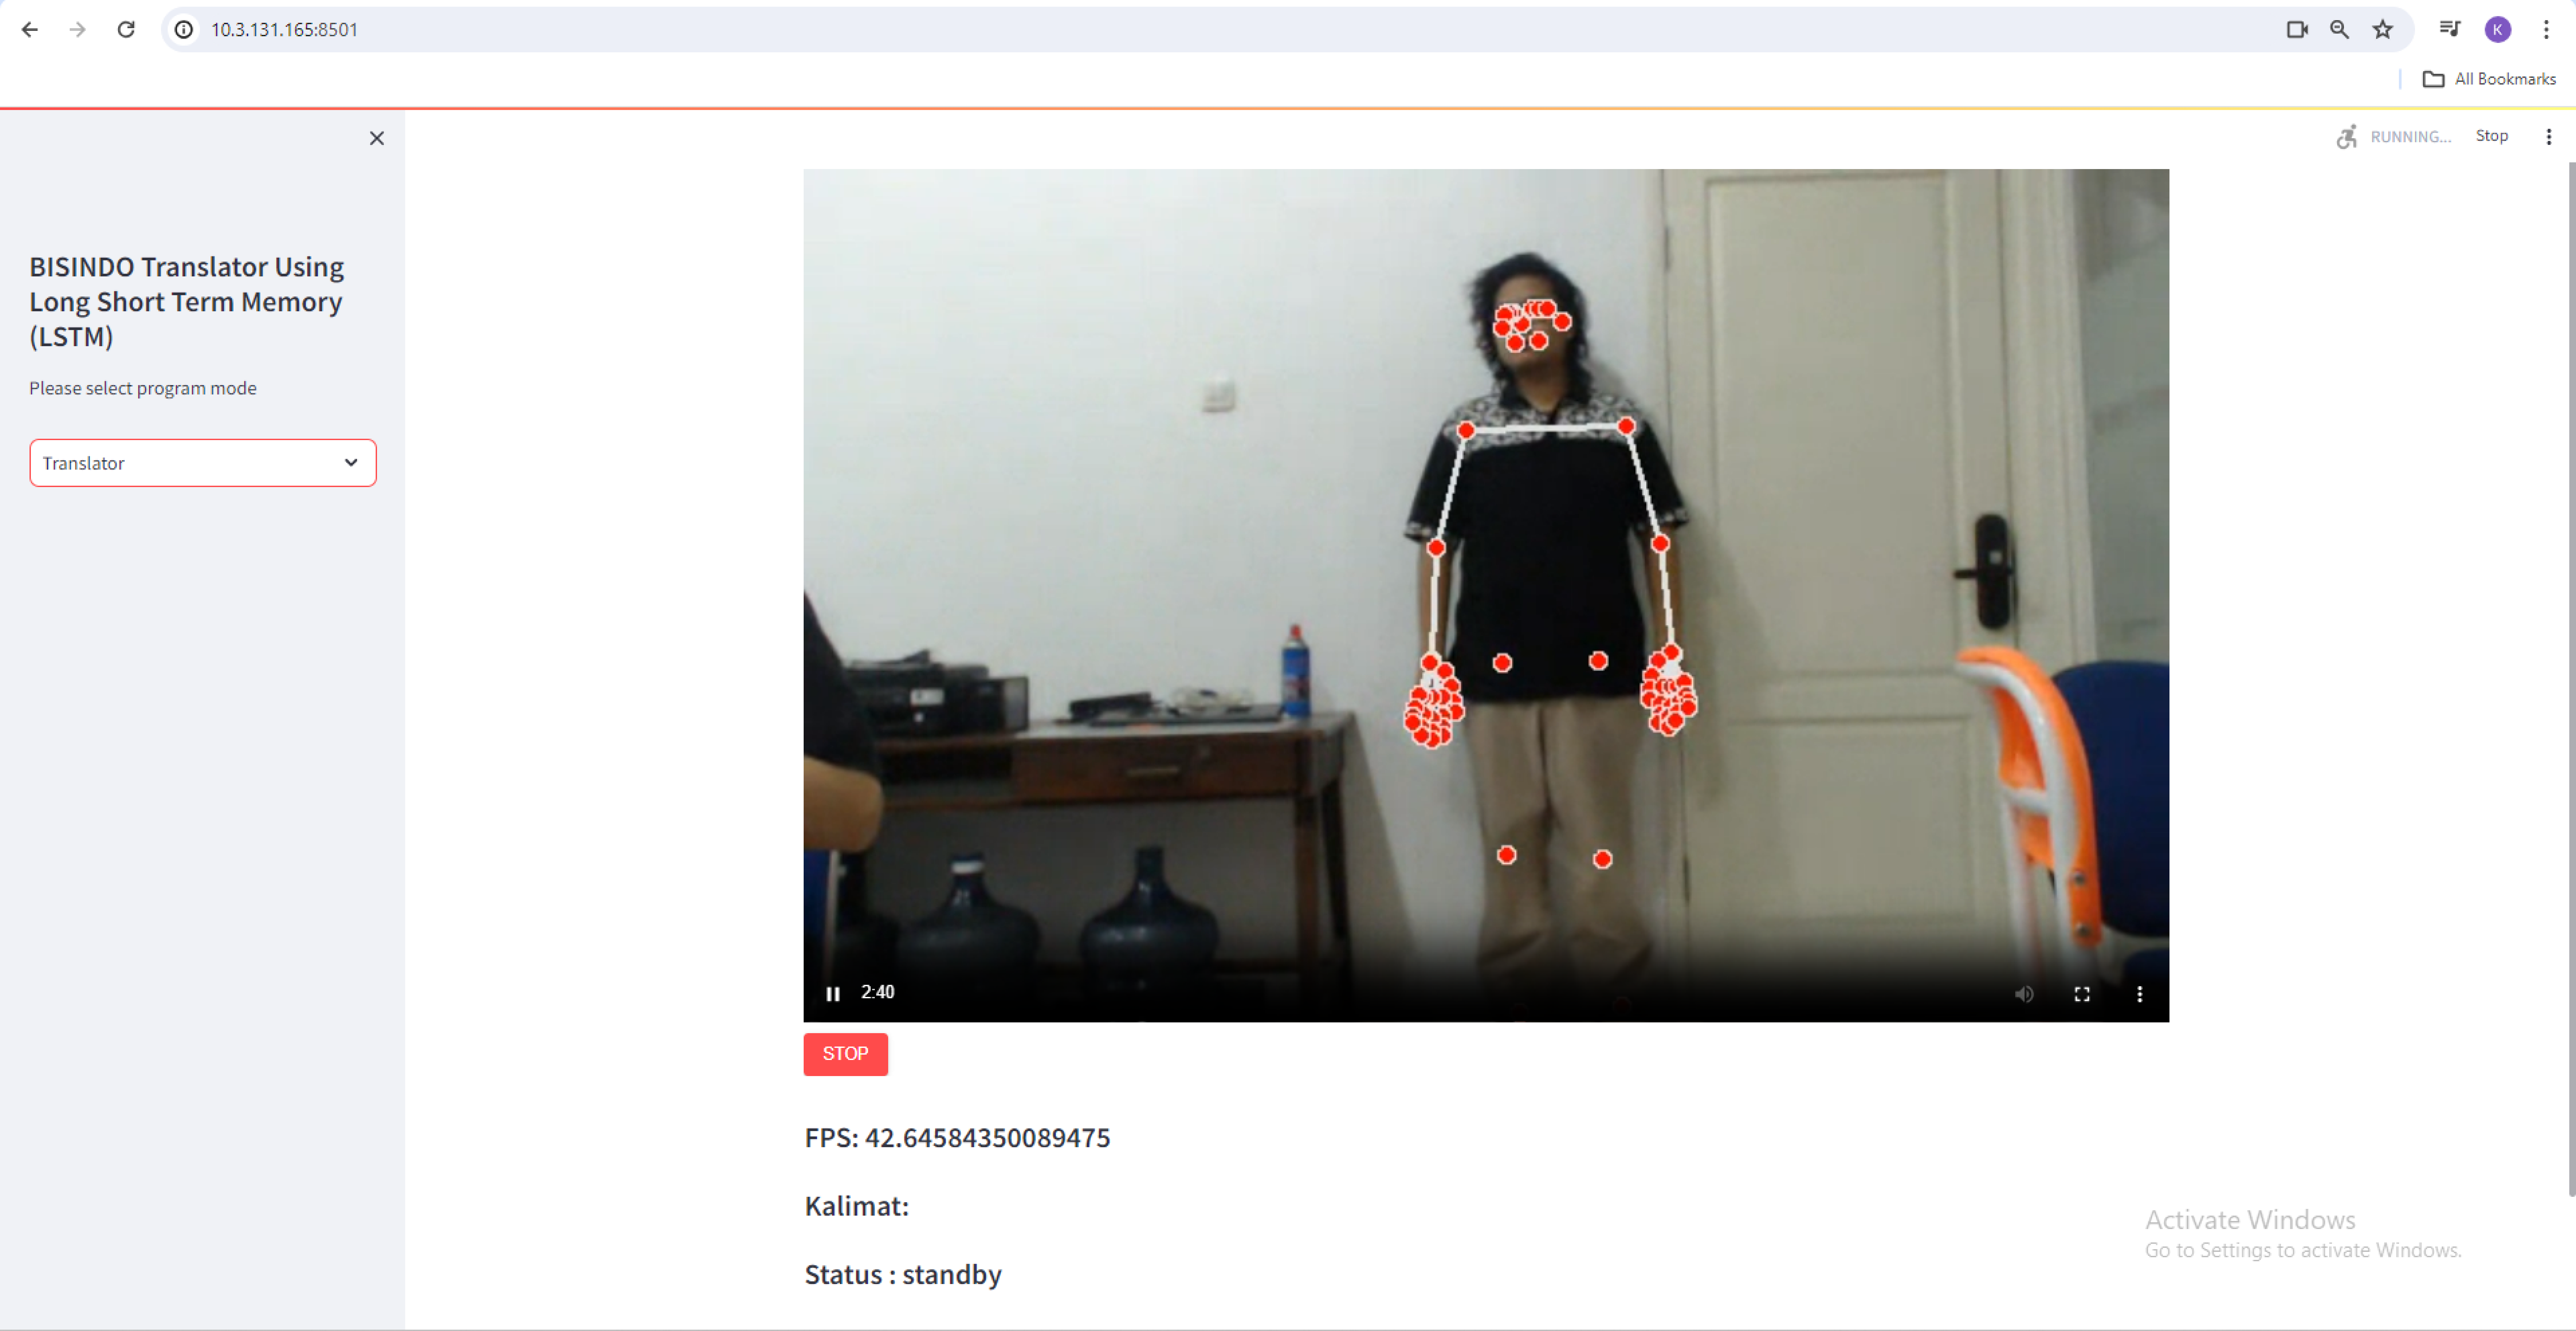
\includegraphics[scale=0.12]{gambar/bab3-layoutweb.png}
 
    \caption{Hasil Pengujian Sistem}
    \label{fig:layoutweb}
\end{figure}